\documentclass{article}
\usepackage{minted, graphicx, amsfonts, amssymb, amsmath, amsthm, float, subcaption} % Required for inserting images
\usepackage[english]{babel}
\usepackage[letterpaper,top=2cm,bottom=2cm,left=3cm,right=3cm,marginparwidth=1.75cm]{geometry}

\title{EE132 Lab 4}
\author{Andre Winkel, Russell Yang}
\date{\today}

\begin{document}
\maketitle

\begin{abstract}
    In this lab, we will analyze and implement first-order transfer functions to perform the bump test. We will derive our parameters for the transfer function from the bump test, which we will implement using Simulink. Doing so will allow us find the steady-state gain and time constant. We will then verify our derived parameters by implementing our transfer function and comparing directly to the encoder output.
\end{abstract}

\section{System built} 
\begin{figure} [H]
    \centering
    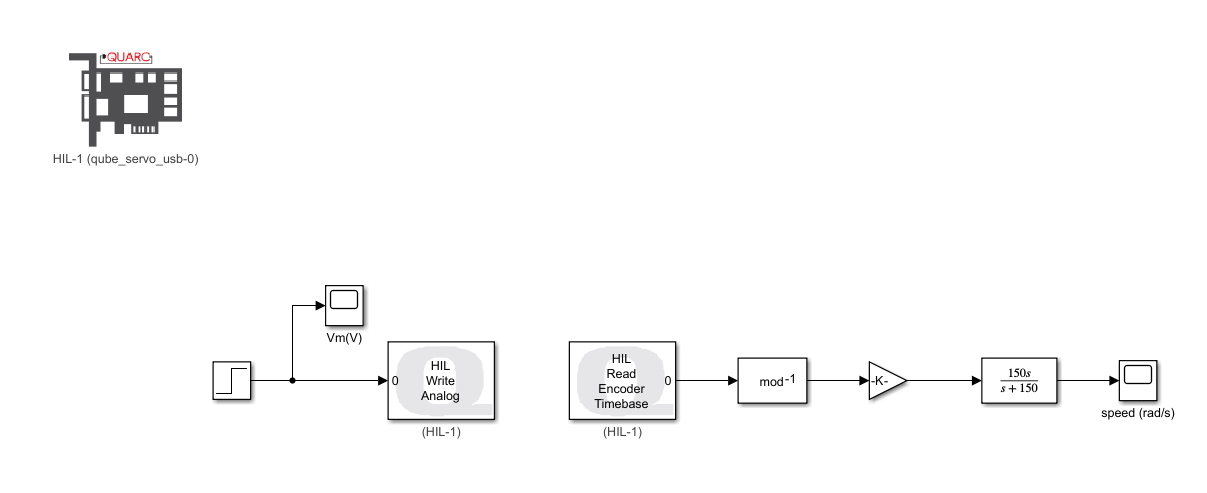
\includegraphics[width=0.75\linewidth]{system1.png}
    \caption{Simulink model constructed for analysis}
    \label{fig:1}
\end{figure}
\begin{figure} [H]
    \centering
    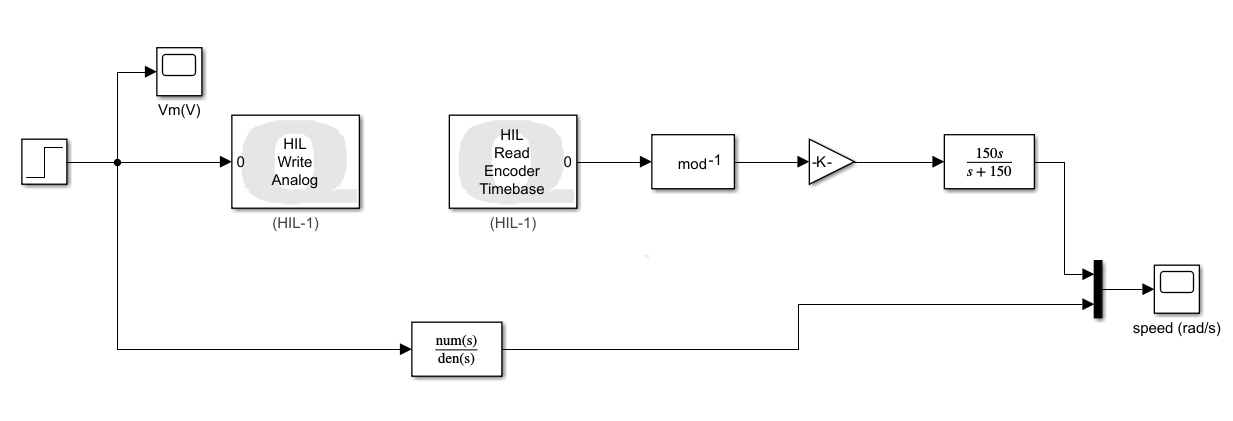
\includegraphics[width=0.75\linewidth]{system2.png}
    \caption{Simulink model constructed for verification}
    \label{fig:2}
\end{figure}

\section{In-Lab exercises and Results}
\subsection{Servo step response}
Running the QUARC controller to apply a 2V step to the servo, we observe the following scope response:
\begin{figure}[H]
    \centering
    \begin{subfigure}[b]{0.45\linewidth}
        \centering
        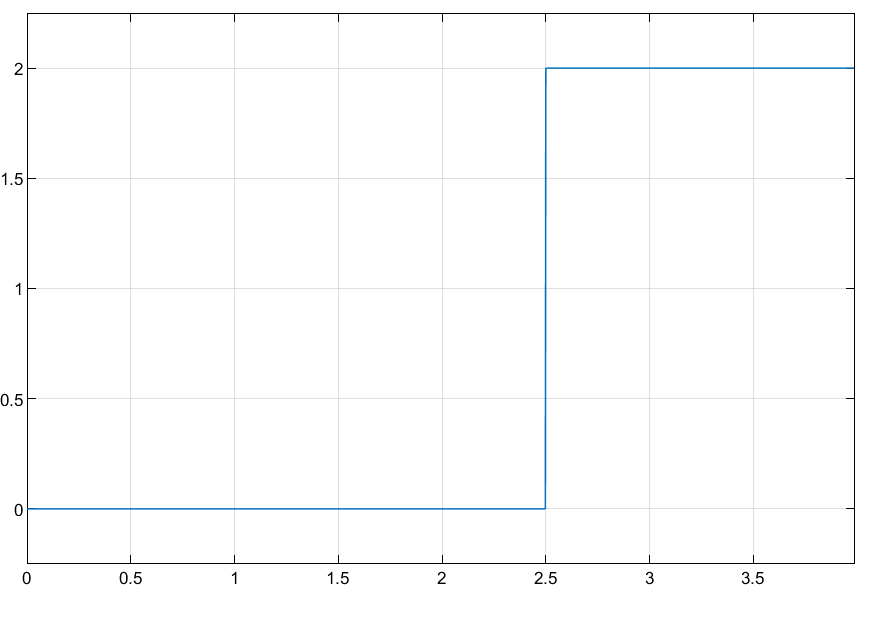
\includegraphics[width=\linewidth]{vm1.png}
        \caption{Motor voltage}
        \label{fig:motorvoltage}
    \end{subfigure}
    \hfill
    \begin{subfigure}[b]{0.45\linewidth}
        \centering
        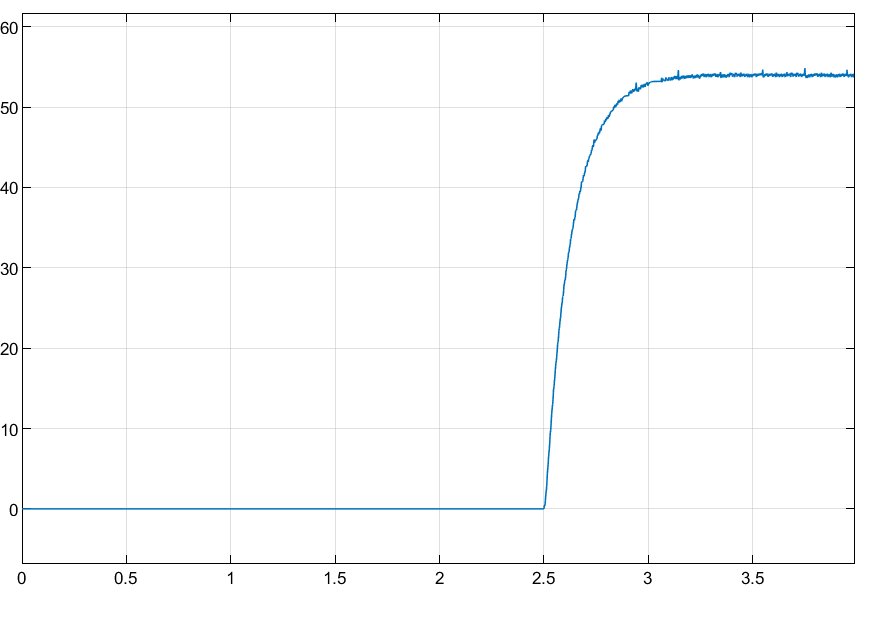
\includegraphics[width=\linewidth]{wm1.png}
        \caption{Load speed}
        \label{fig:loadspeed}
    \end{subfigure}
    \caption{System response to a 2V step}
    \label{fig:2vstep}
\end{figure}

\subsection{Deriving model parameters}
Recalling, the time constant of a system $\tau$ is defined as the time it takes the system to respond to the application of a step input to reach a factor of $1-\frac{1}{e}$ of its steady-state value. We can determine the steady-state value by observing the rightmost end of the load speed, which we determined to be approximately $53.5\frac{rad}{s}$. This then implies
\begin{equation}
    y(t_1)=(1-\frac{1}{e})\Delta y+y_0,
\end{equation}
where $\Delta y$ is the steady-state value. We can then observe the plot using \verb|ginput| to determine $t_1$, and subsequently $\tau$, where
\begin{equation}
    \tau=t_1-t_0
\end{equation}
and $t_0=2.5$, the time at which the step input is applied. We can find our value for $\tau$ following the above procedures by importing our data values into MATLAB and observing the plot.
\begin{minted}[frame=single, fontsize=\small, linenos, bgcolor=white]{matlab}
plot(data_wm.time, data_wm.signals.values)
y1 = 53.5*(1-1/exp(1))
k = 53.5/2
t0 = 2.5
[t1, y] = ginput(1)
t1 = 2.63
tau = t1 - t0
\end{minted}
Here, we find that
\begin{equation}
    y_1\approx33.8184,
\end{equation}
and observing the plot,
\begin{equation}
    t_1 = 2.63.
\end{equation}
This then means that
\begin{equation}
    \tau = 2.63-2.5=0.13.
\end{equation}
Additionally, $K$ is the model steady-state gain, which gives us
\begin{equation}
    K=\frac{\Delta y}{\Delta u} = \frac{53.5}{2}=26.75.
\end{equation}

\subsection{Verifying results}
Implementing our derived values into our voltage-to-speed transfer function, we obtain
\begin{equation}
    \frac{\Omega_m(s)}{V_m(s)}=\frac{K}{\tau s+1}=\frac{26.75}{0.13s+1}
\end{equation}
as our transfer function. Implementing this in Simulink and comparing with our measured results, we observe the following response:
\begin{figure}
    \centering
    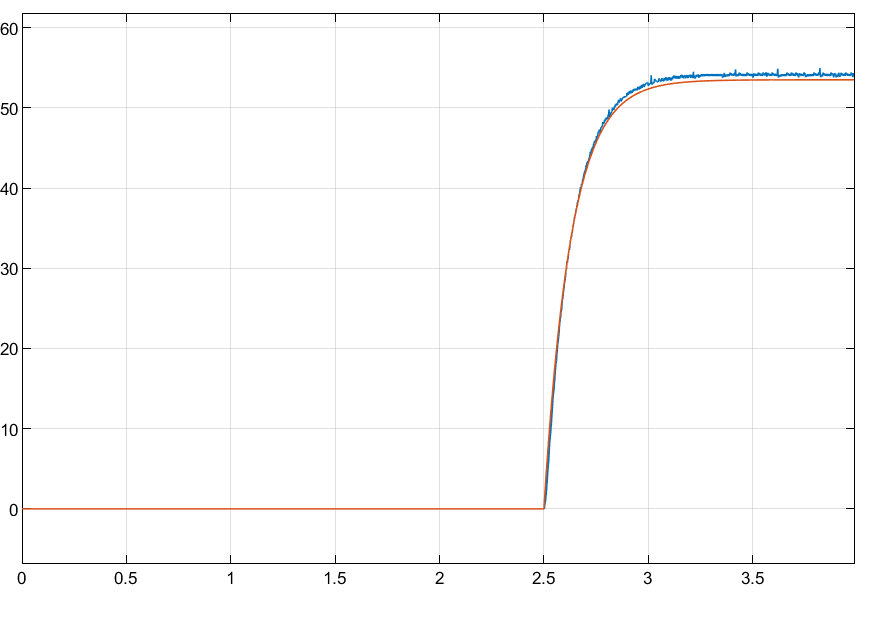
\includegraphics[width=0.5\linewidth]{wm2.png}
    \caption{Load speed and transfer function with step}
    \label{fig:analysis}
\end{figure}

\subsection{Verifying result accuracy}
We can directly observe that our derived values implemented into our transfer function nearly identically model the measured load speed. This is demonstrated in Figure 4, where we can observe two nearly identical lines representing the speed. Therefore, we can determine our derived values must be accurate.

\section{Analysis}
Through our exercises and analysis of our system, we were able to directly derive our values for the open-loop transfer function representation of the system. We did so by analyzing and observing the data we collected directly from our measured encoder values before implementing them into our voltage-to-speed transfer function. As shown in equations (5), (6), and (7), our obtained values were $K=26.75$, $\tau=0.13$, and our resultant transfer function is $\frac{26.75}{0.13s+1}$. As shown in Figure 4, this transfer function is a very accurate representation of the original system. One of the few issues we encountered during our analysis was transferring our values to our MATLAB program for observation and extracting data. Subsequently, our unorthodox method of "looking at the data" was likely what obtained our very slight inaccuracy for the max value of the transfer function with the step input, shown by the small discrepancy between the two plotted lines in Figure 4 as $t\to\infty$, where our calculated transfer function is slightly less than that of the original system. However, this is likely easily modifiable by slightly increasing our initial estimated $\Delta y$ value.

\section{Conclusion}
During this lab, we were able to obtain data through our Simulink encoder measurements, subsequently analyzing said data in order to extract important values. Through doing so, we were able to calculate and obtain the necessary values to implement in our voltage-to-speed transfer function, which resulted in an accurate representation of the original system. We directly verified our transfer function's accuracy by directly comparing with the original system, subsequently verifying its accuracy.

\end{document}